\documentclass[10pt]{exam}
\usepackage[hon]{template-for-exam}
\usepackage{tikz}
\usetikzlibrary{
  calc,
  patterns,
  decorations.pathmorphing,
  decorations.markings,
  arrows,
  shapes,
  positioning,
  math,
  intersections,
  fadings
}

\title{Snell's Law (of Refraction)}
\author{Rohrbach}
\date{\today}

\begin{document}
\maketitle


\tikzfading[
  name=fade out,
  inner color=transparent!0,
  outer color=transparent!50]

\noindent
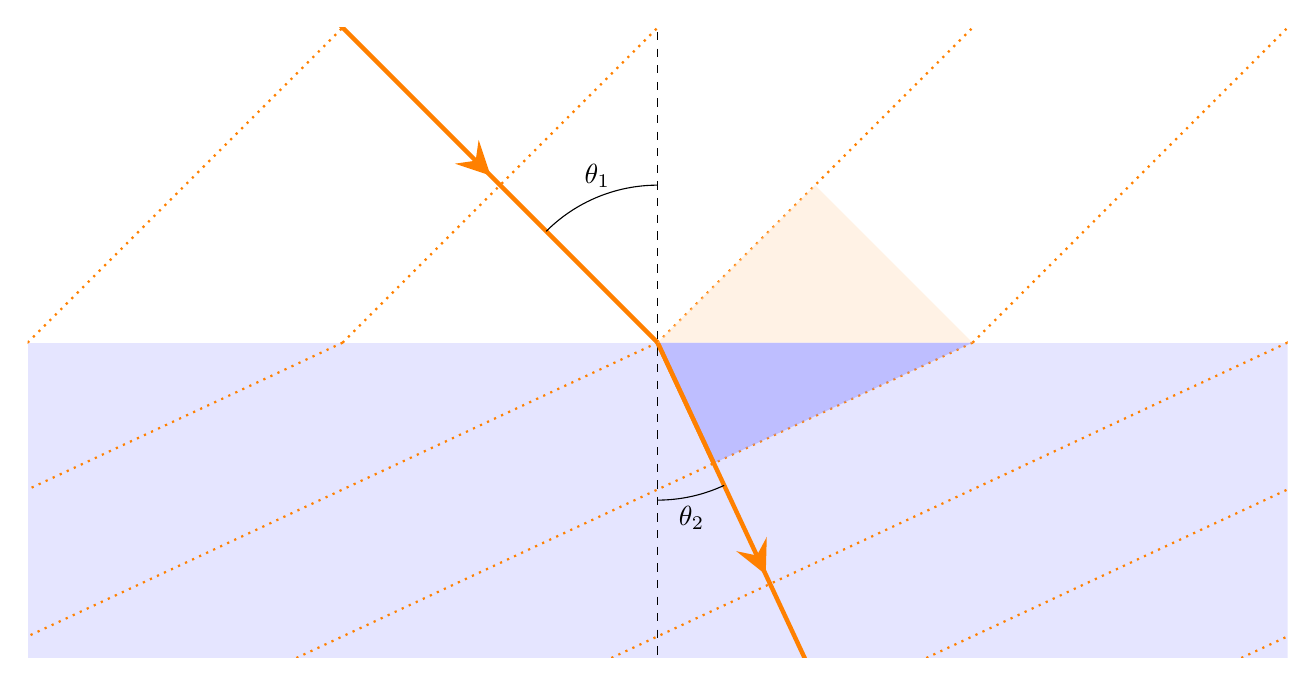
\begin{tikzpicture}
  \tikzstyle{directed}=
    [postaction={decorate,decoration={markings,
    mark=at position .65 with {\arrow[scale=2]{stealth}}}}]
  \tikzstyle{reverse directed}=
    [postaction={decorate,decoration={markings,
    mark=at position .5 with {\arrowreversed[scale=2]{stealth}}}}]

  \tikzstyle{ray}=[orange,ultra thick]
  \tikzstyle{normal}=[dashed]
  \tikzstyle{wavefront}=[dotted,orange,thick]
  \tikzstyle{glass}=[blue!10]



  \def\incident{135}
  \def\refracted{-65}

  \clip (-8,-4) rectangle (8,4);
  \fill[glass] (-8,0) rectangle (8,-5);
  \draw[ray,reverse directed] 
    (0,0) -- (\incident:6);
  \draw[ray,directed,name path=refr] 
    (0,0) -- (\refracted:5);
  \draw[normal] (0,5) -- (0,-5);
  
  \draw (0,2) arc (90:\incident:2)
    node[midway,above] {$\theta_1$};
  \draw (0,-2) arc (-90:\refracted:2)
    node[midway,below] {$\theta_2$};


  \tikzmath{
    \wavefrontinc = \incident-90;
    \wavefrontref = \refracted+90;
  }
  \foreach \i in {-8,-4,...,16}{
    \draw[wavefront] (\i,0) -- ++(\wavefrontinc:20);
    \draw[wavefront] (\i,0) -- ++(\wavefrontref:-20);
  }

  \path[name path=wf] (4,0) -- ++(\wavefrontref:-20);
  \path[name path=wf 2] (0,0) -- ++(\wavefrontinc:20);
  \path[name path=inc 2] (4,0) -- ++(\incident:10);


  \fill[
    name intersections={of=refr and wf},
    blue!40,
    semitransparent,
    %path fading=fade out,
    ] 
      (0,0) -- (4,0) -- 
      (intersection-1) coordinate (v) -- cycle; 
  %\draw[wavefront] (4,0) -- ++(\wavefrontref:-20);
  \draw[ray] (0,0) -- (v);

  \fill[
    name intersections={of=inc 2 and wf 2},
    orange!20,
    semitransparent,
    %path fading=fade out,
    ] 
      (0,0) -- (4,0) -- (intersection-1) -- cycle; 

  
\end{tikzpicture}

\pagebreak

\section*{Practice Problems}

\begin{questions}
  \question 
    The speed of light in ice is \SI{2.29e8}{\meter\per\second}.  What is the index of refraction of ice?
    \vs

  \question
    A flashlight beam strikes the surface of a pane of glass (n=1.56) at an angle of $67^\circ$ to the normal.  What is the angle of refraction?
    \vs

  \question
    A diver shines a flashlight upward from beneath the water ($n=1.33$) at an angle $35^\circ$ to the vertical.  At what angle does the light leave the water?
    \vs

  \question
    What is the critical angle for the interface between acryllic plastic ($n=1.49$) and water ($n=1.33$).  To be internally reflected, the light must start out in which medium?
    \vs
 
\end{questions}

\end{document}